% Chapter Template

\chapter{Development of An Efficient 2D-Ewald Summation Method}

\label{Chapter3}

\lhead{Chapter 3. \emph{Development of An Efficient 2D-Ewald Summation Method}} 
In the case of a two-dimensional periodic system, the summation over the $m_z$ component in Eq.~(\ref{eq:coul}) is omitted, which alters the Ewald formulation relative to the fully periodic (3D) case and leads to a Fourier integral, thereby increasing the computational cost. In this chapter, we propose to retain this summation as in the three-dimensional periodic system, and introduce a top-hat function, which acts as a filter for removing the contributions that are not from the 2D-Ewald summation. This function is set up so that it eliminates contribution from periodic images along the $z$-direction, while retaining the efficiency of 3D-Ewald summation in the reciprocal space. 
 
\section{Top-hat function}
\begin{figure}[]% if you want to fix the position of this image, add H inside the []
    \centering
    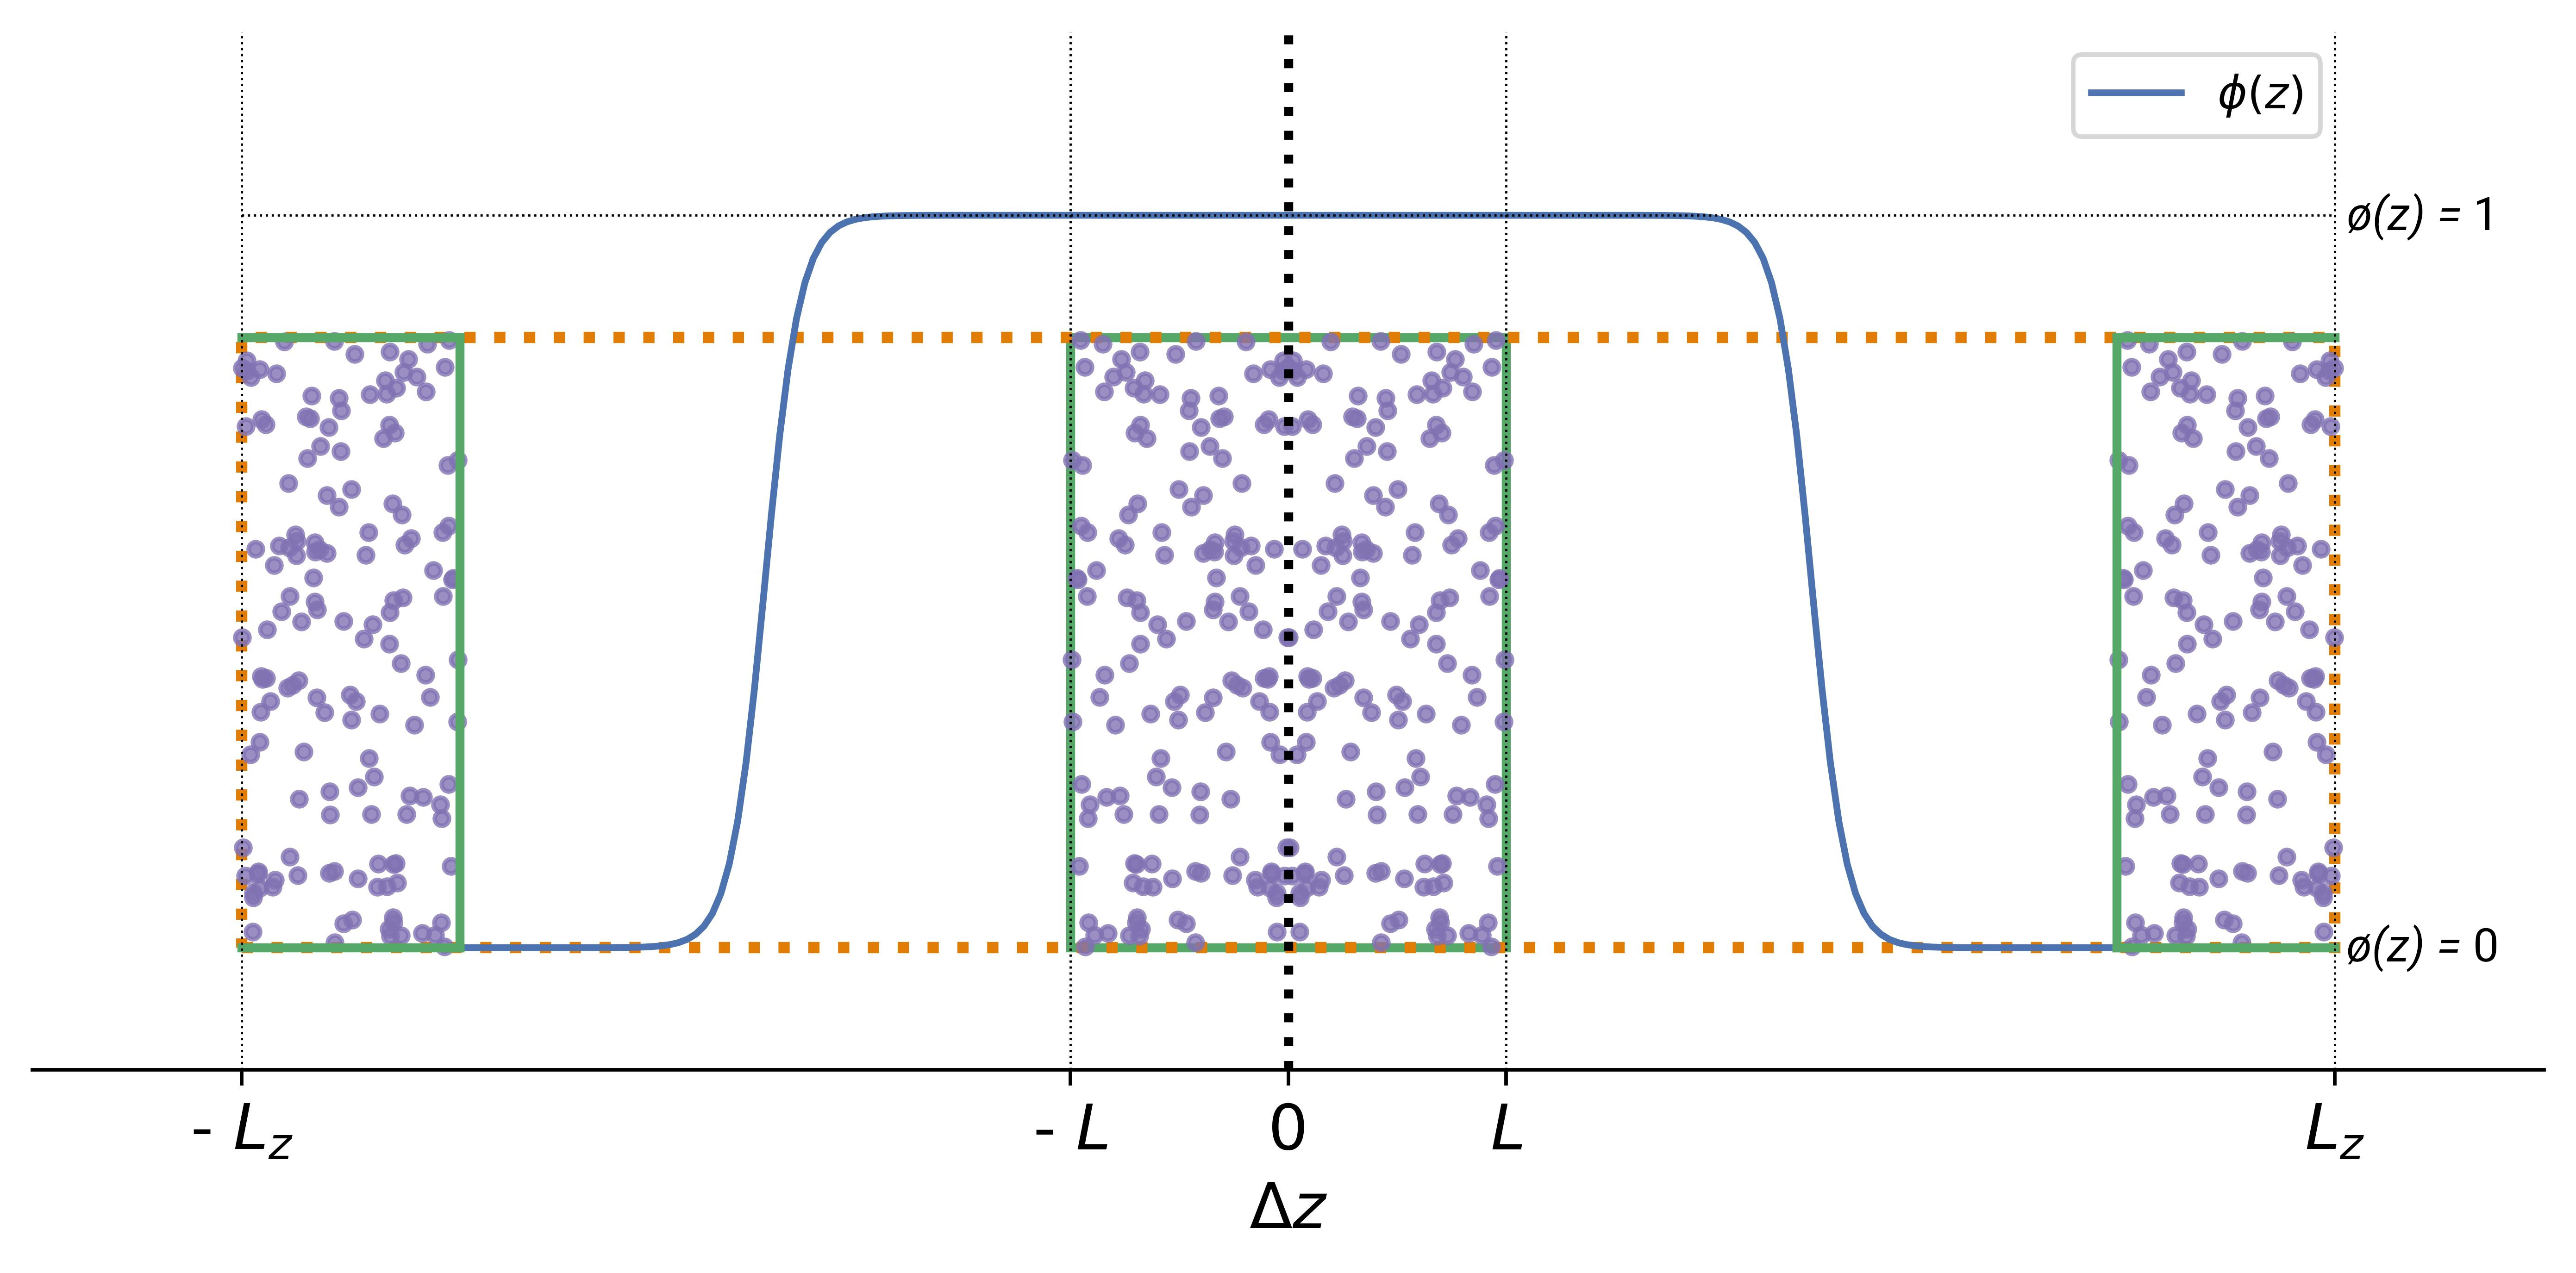
\includegraphics[width=\linewidth]{images/simulationcell.jpg}
    \caption{Schematic figure showing the basic idea of the correction.}
    \label{fig:simulation_cell}
\end{figure}
We begin by elucidating the basic idea of the method and then formulating the rigorous mathematics.
To exclude the system's interactions along the $z$-direction, a spatially dependent window function $\phi(z)$ is introduced. The simplest version of $\phi(z)$ is a top-hat function defined as:
\begin{flalign*} 
    \phi(z) = 
    \begin{cases} 
        1 & \text{if } z \in (-\frac{L_z}{2}, \frac{L_z}{2}) \\
        0 & \text{otherwise}
    \end{cases}
\end{flalign*}
While this function is straightforward, its sharp discontinuities at the edges can introduce numerical artefacts, especially in methods sensitive to derivatives or smoothness (e.g., force field calculations). To address this, the discontinuous top-hat function is replaced with a smooth approximation that retains the essential features of the original function while providing a differentiable and numerically stable function.
The smoothed version of $\phi(z)$ is expressed as:
\begin{flalign}
    \phi(z) &= \frac{1}{1+ exp(-\gamma(0.5L_z+z))} + \frac{1}{1+ exp(-\gamma(0.5L_z-z))} -1 \label{eq:1}
\end{flalign}
This function uses a linear combination of two Fermi functions (sigmoid functions) to obtain a symmetrical function about the origin. The positive constant \textbf{$\gamma$} determines the steepness of the top-hat around the edges. The behaviour of $\phi(z)$ Eq. (\ref{eq:1}) is shown in Fig.~(\ref{fig:tophat}). Other forms of the top-hat functions can also be used; some examples are as follows:
\begin{flalign}
        \phi(z) &= \frac{1}{2}[ \tanh(\gamma(x + 0.5L)) -\tanh(\gamma(x - 0.5L)) ] \\
        \phi(z) &= \frac{2}{\pi}\left[ \arctan \left( e^{\gamma (-x + 0.5L)} \right) + \arctan \left( e^{\gamma (x + 0.5L)} \right) \right]- 1 
\end{flalign}
\begin{figure}[htbp]
    \centering
    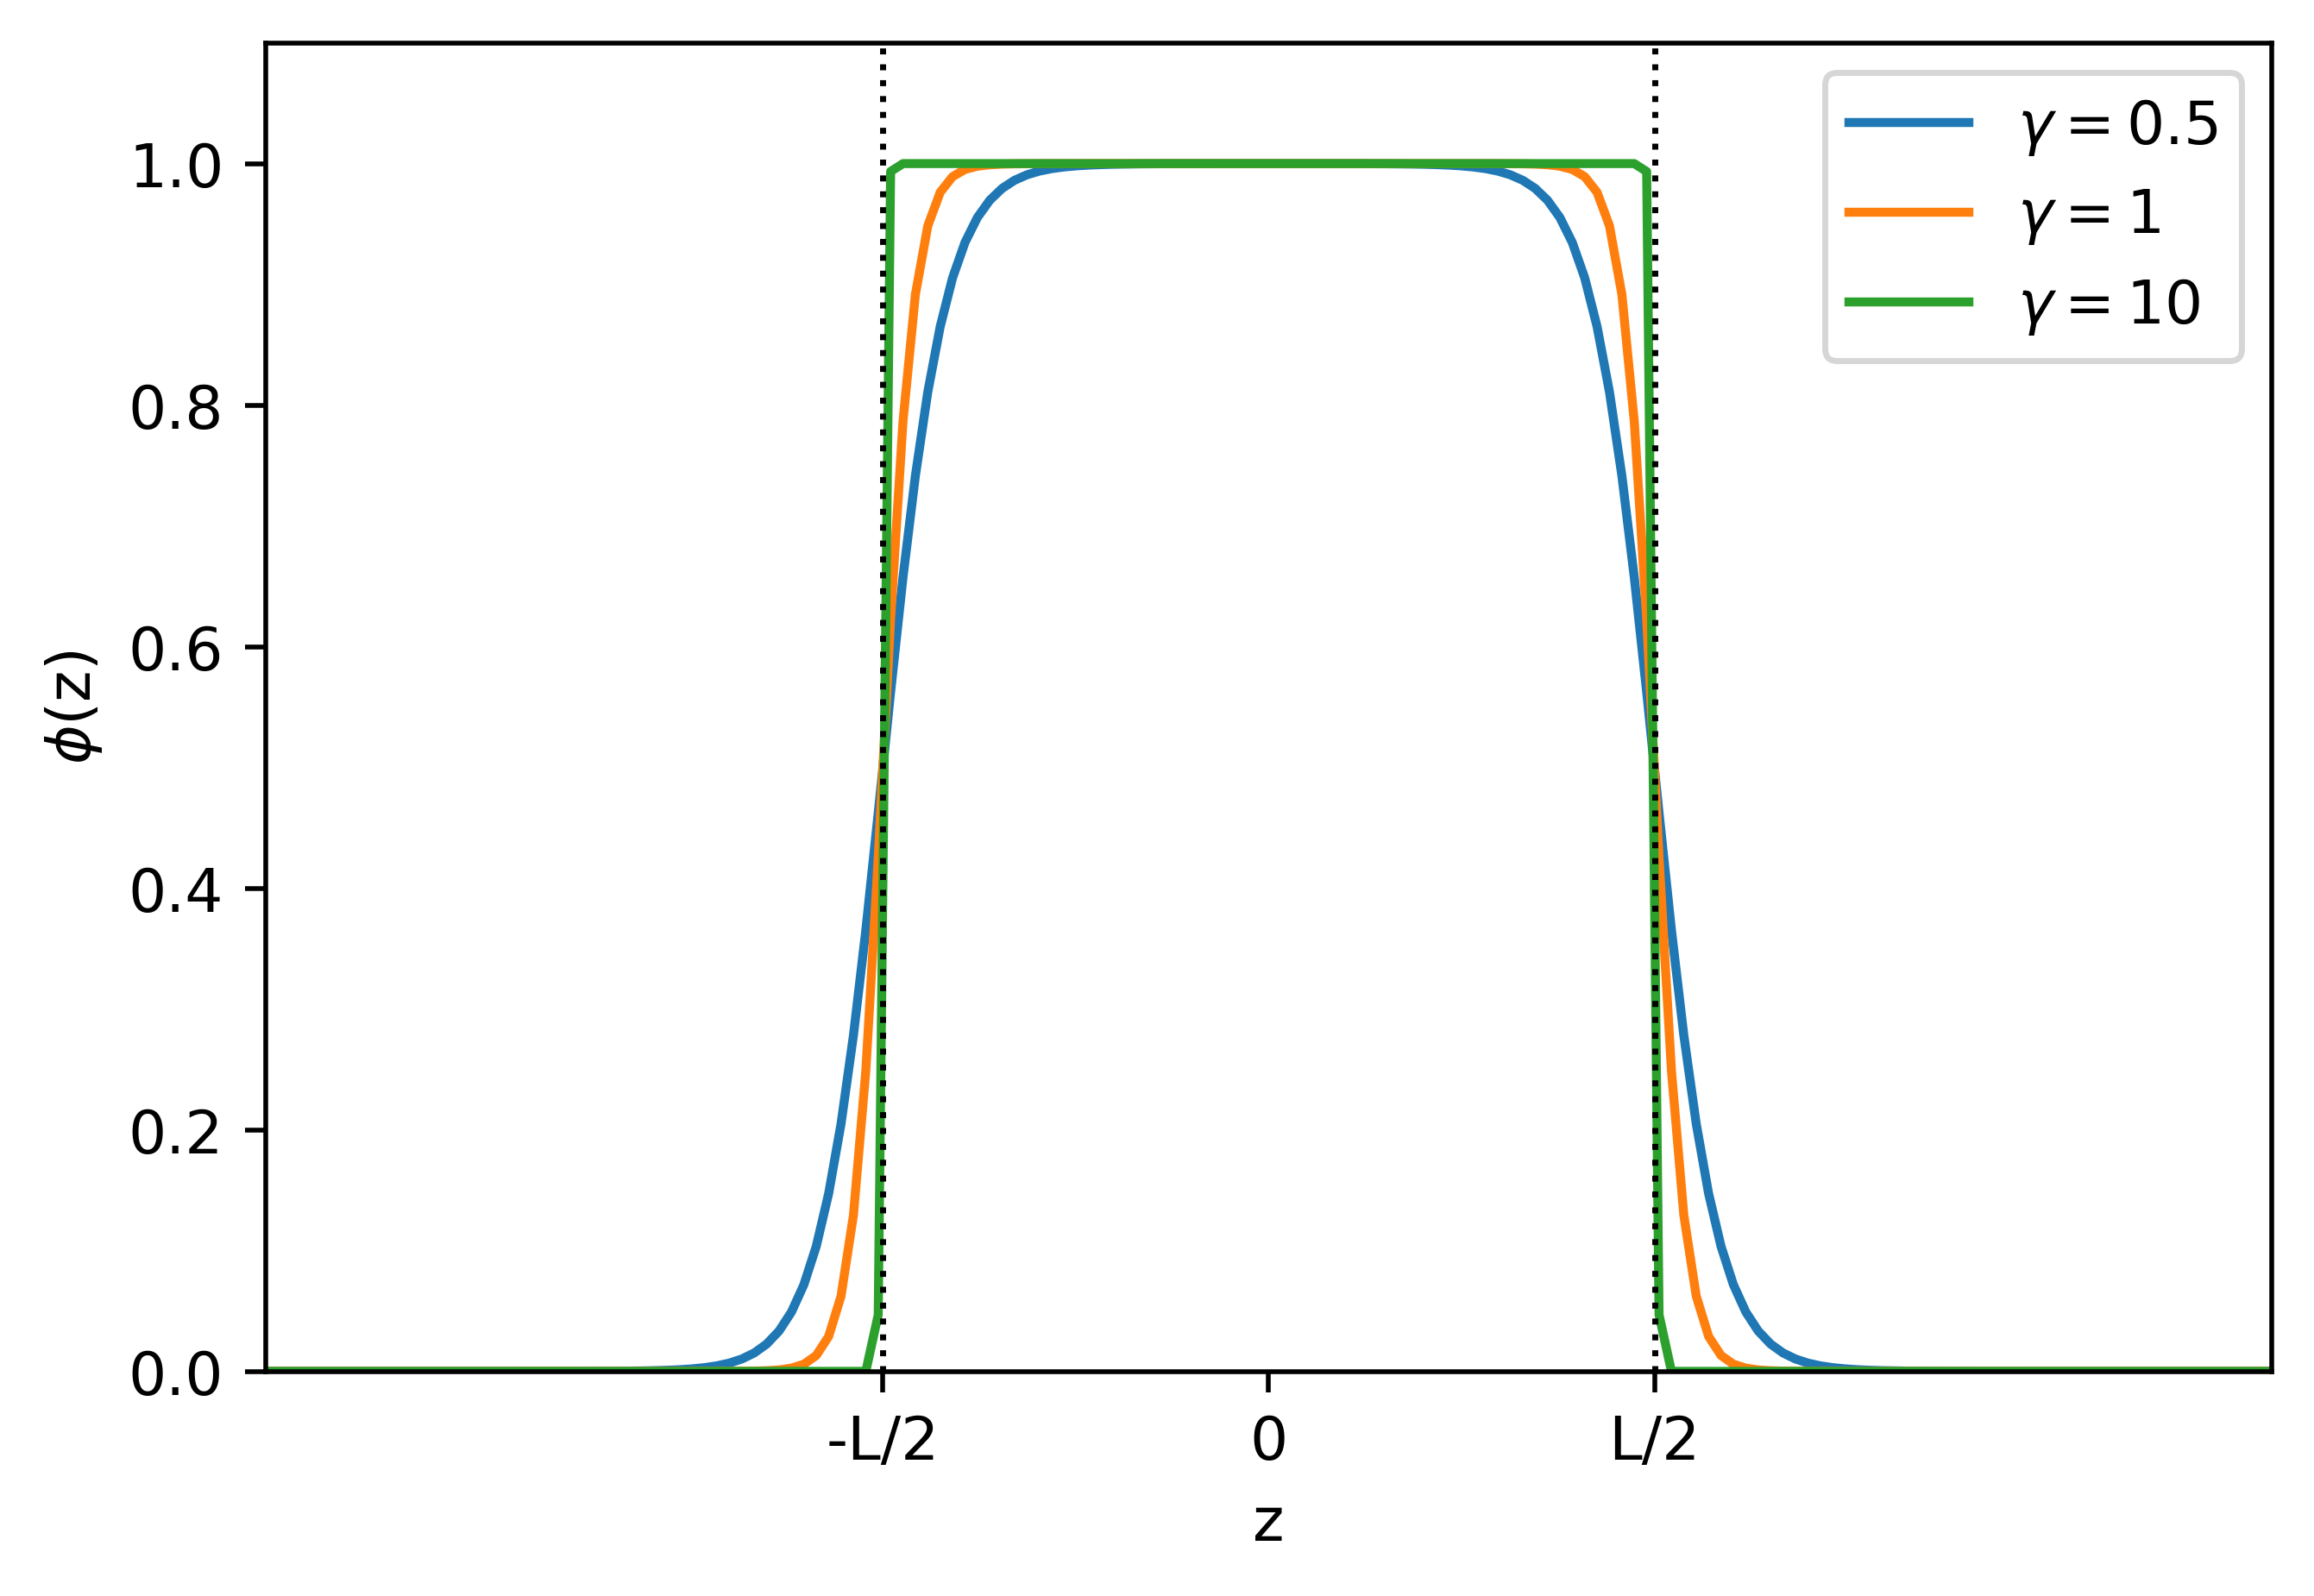
\includegraphics[width=0.8\linewidth]{images/TopHat2.png}
    \caption{Visualisation of the top-hat function for different $\gamma$. As $\gamma$ increases, the function transitions more sharply at the boundaries, approaching an ideal window function.}
    % \parbox{0.5\linewidth}{\justifying \caption{Visualization of top-hat function for different $\gamma$. As $\gamma$ increases, the function transitions more sharply at the boundaries, approaching an ideal window function.}}
    \label{fig:tophat}
\end{figure}
A vacuum is introduced within the simulation cell along the $z$-axis to accomplish the above, resulting in a total side length of $ L_z$. Ideally, this length must be long enough for the next periodic image to lie in the region where this function $\phi(z)$ is precisely zero. 

\section{Mathematical Details}
To evaluate the long-range contribution to the electrostatic energy in a two-dimensional (2D) periodic system, we begin with the derivation of the standard three-dimensional (3D) Ewald summation expression. A top-hat function, denoted by $\phi(z)$, is introduced to eliminate the influence of periodic images along the non-periodic $z$-direction. This function ensures that only the electrostatic interactions within the simulation box along the $z$-direction are retained, effectively reducing the system to 2D while preserving the 3D summation structure and efficiency.

The long-range part of the Coulomb interaction, initially expressed as $\frac{\text{erf}(\alpha r)}{r}$, is converted into an integral form using the identity\cite{erf}:
$$
\frac{\text{erf}(\alpha r)}{r} = \frac{2}{\sqrt{\pi}} \int_0^\alpha e^{-r^2 t^2} dt.
$$
This transformation separates the exponential term into components along the $x$, $y$, and $z$ directions.
\begin{flalign}
    \nonumber(4\pi\epsilon_o)U^{LR} & = \frac{1}{2}\sum_{\vec{M}=-\infty}^{\infty}\sum_{i=1}^{n_p}\sum_{j=1}^{n_p}q_i q_j \frac{{erf}(\alpha|\vec{r_i}-\vec{r_j}+\vec{M}.\vec{L}|)}{|\vec{r_i}-\vec{r_j}+\vec{M}.\vec{L}|} \,\phi(z_{ij}+m_zL_z)\quad\quad\quad\quad
\end{flalign}
\begin{flalign}
    \nonumber\quad\quad\quad\quad\quad& = \frac{1}{2}\sum_{\vec{M}=-\infty}^{\infty}\sum_{i=1}^{n_p}\sum_{j=1}^{n_p}\frac{2q_i q_j}{\sqrt{\pi}}\int_{0}^{\alpha}dt\,  {exp}(-|\vec{r_i}-\vec{r_j}+\vec{M}.\vec{L}|^2 t^2)\,\phi(z_{ij}+m_zL_z)\\
    \nonumber &=\frac{1}{2}\sum_{\vec{M}=-\infty}^{\infty}\sum_{i=1}^{n_p}\sum_{j=1}^{n_p}\frac{2q_i q_j}{\sqrt{\pi}}\int_{0}^{\alpha}dt\,  {exp}\left[-(x_{ij}+m_xL_x)^2 t^2\right] \\
    &\quad\quad\quad\times{exp}\left[-(y_{ij}+m_yL_y)^2 t^2\right]\times{exp}\left[-(z_{ij}+m_zL_z)^2 t^2\right] \, \phi(z_{ij}+m_zL_z)
\end{flalign}
The Poisson summation formula~\cite{cordoba1988formule} converts the expression from real to reciprocal space. The detailed derivation of this transformation is provided in the Appendix~\ref{AppendixA}.
\begin{flalign}
    \nonumber(4\pi\epsilon_o)U^{LR}& =\frac{\sqrt{\pi}}{L_xL_y}\sum_{\vec{\mathbf{k}}=-\infty}^{\infty}\sum_{j=1}^{n_p}\sum_{k=1}^{n_p}q_j q_k \int_{0}^{\alpha}\frac{dt}{t^2}\,{exp}\left(\frac{-\pi^2k_x^2}{L_x^2t^2}+i \frac{2\pi k_xx_{ij}}{L_x}\right)
    \\&\quad\quad\quad
    \times\,{exp}\left(\frac{-\pi^2k_y^2}{L_y^2t^2}+i\frac{2\pi k_yy_{ij}}{L_y}\right)\times C_{k_z}(t)\,{ exp}\left(i\frac{2\pi k_zz_{ij}}{L_z}\right)\label{eq:transform}
\end{flalign}
The function $C_{k_z}(t)$ is given by
\begin{flalign}
     C_{k_z}(t) &=\frac{1}{L_z}\int_{-\infty}^{\infty}ds\,exp(-i\frac{2\pi n s}{L_z})\, exp(-s^2t^2)\, \phi(s) \label{eq:Cz}
     % \\ &=\frac{1}{L_z}\int_{-\infty}^{\infty}ds\hspace{1mm}exp(-i\frac{2\pi n s}{L_z})\hspace{1mm} exp(-s^2t^2)\left[\frac{1}{1+ exp(-\gamma(0.5L_z+s))} + \frac{1}{1+ exp(-\gamma(0.5L_z-s))} -1\right]
\end{flalign}
Eq. (\ref{eq:transform}) is written using the reciprocal vector formulation as
\begin{flalign*}
    \nonumber(4\pi\epsilon_o)U^{LR}& =\frac{\sqrt{\pi}}{L_xL_y}\sum_{\vec{\mathbf{k}}=-\infty}^{\infty}\sum_{i=1}^{n_p}\sum_{j=1}^{n_p}q_i q_j\int_{0}^{\alpha}\frac{dt}{t^2}\,{ exp}\left[i\vec G.(\vec r_i-\vec r_j)\right]\times C_{k_z}(t)\,{ exp}\left(\frac{-1}{4t^2}|\vec G|_{xy}^2\right)\\
    &=\frac{\sqrt{\pi}}{L_xL_y}\sum_{\vec{\mathbf{k}}=-\infty}^{\infty}\left[ \int_{0}^{\alpha}\frac{dt}{t^2}C_{k_z}(t)\,{exp}\left(\frac{-1}{4t^2}|\vec G|_{xy}^2\right)\right]\sum_{j=1}^{n_p}\sum_{k=1}^{n_p}q_i q_j\,{ exp}\left[i\vec G.(\vec r_i-\vec r_j)\right]
\end{flalign*}
The double summation over indices $j$ and $i$ is reformulated as a single summation incorporating the structure factor Eq.\ (\ref{eq:structurefactor}).
Hence, the final expression for the two-dimensional Ewald summation takes the form
\begin{flalign}
    (4\pi\epsilon_o)U^{LR}& =\frac{\sqrt{\pi}}{L_xL_y}\sum_{\vec{{k}}=-\infty}^{\infty}{}^\prime\left[ \int_{0}^{\alpha}\frac{dt}{t^2}C_{k_z}(t){exp}\left(\frac{-1}{4t^2}|\vec G|_{xy}^2\right)\right] |\,S(\vec G)\,|^2
\end{flalign}
The prime symbol (${}^\prime$) indicates that the $\vec{k} = 0$ component is omitted from the summation, since it vanishes when the system is electrically neutral, that is, when the total charge sums to zero.
Define $\Lambda(p_1,p_2,p_3)$ as
\begin{flalign}
    \nonumber \Lambda(p_x,p_y,p_z) &= \frac{\sqrt{\pi}}{L_xL_y}\sum_{\vec{\mathbf{k}}=-\infty}^{\infty}{}^\prime \left[ \int_{0}^{\alpha}\frac{dt}{t^2}C_{k_z}(t){exp}\left(\frac{-1}{4t^2}|\vec G|_{xy}^2\right)\right] 
    \\&\times B_{3D}(k_x,k_y,k_z)\times \exp\left( i \frac{2\pi k_x p_x}{K_x} + i \frac{2\pi k_y p_y}{K_y} + i \frac{2\pi k_z p_z}{K_z} \right)
    \\&=\mathcal{F}_{3D}(E_{2D-M}.B_{3D})(p_x,p_y,p_z)
\end{flalign}
where the new screening factor array $E_{2D-M}$ is defined as
\begin{flalign}
    E_{2D-M}(k_x,k_y,k_z) &= \frac{\sqrt{\pi}}{L_xL_y}\left[ \int_{0}^{\alpha}\frac{dt}{t^2}C_{k_z}(t){exp}\left(\frac{-1}{4t^2}|\vec G|_{xy}^2\right)\right] 
\end{flalign}
Note that $E_{2D-M}\cdot B_{3D}(k_x,k_y,k_z) = \mathcal{F}^{-1}_{3D}(\Lambda)$. 
Furthermore, the structure factor can be efficiently calculated using the smooth particle mesh Ewald (SPME) method by using fast fourier transforms (FFTs).
\begin{flalign}
    \nonumber (4\pi\epsilon_o)U^{LR}  & \approx \frac{\sqrt{\pi}}{L_xL_y}\sum_{\vec{\mathbf{k}}=-\infty}^{\infty}{}^{\prime}\left[ \int_{0}^{\alpha}\frac{dt}{t^2}C_{k_z}(t){exp}\left(\frac{-1}{4t^2}|\vec G|_{xy}^2\right)\right]\,B_{3D}(k_x,k_y,k_z)
    \\& \quad\quad\quad\quad\quad\quad\quad\quad\times \left|\mathcal{F}_{3D}(Q)(k_x,k_y,k_z)\right|^2 \label{eq:newreci2DSPME}\\
    \nonumber&= \sum_{k_x=0}^{K_1-1} \sum_{k_y=0}^{K_2-1} \sum_{k_z=0}^{K_3-1}\mathcal{F}^{-1}_{3D}(\Lambda)(k_x,k_y,k_z)\cdot \cdot \mathcal{F}_{3D}(Q)(k_x,k_y,k_z) \\
    \nonumber &\quad\quad\quad\quad\quad\cdot K_xK_yK_z\,\mathcal{F}^{-1}_{3D}(Q)(k_x,k_y,k_z) \\
    &=\sum_{k_x=0}^{K_1-1} \sum_{k_y=0}^{K_2-1} \sum_{k_z=0}^{K_3-1} Q(k_x,k_y,k_z) \cdot (\Lambda \star Q)(k_x,k_y,k_z)
\end{flalign}
The reciprocal space force is obtained as
\begin{flalign}
    \frac{\partial U^{LR}}{\partial r_{\beta i}} &= 2\sum_{k_x=0}^{K_1-1} \sum_{k_y=0}^{K_2-1} \sum_{k_z=0}^{K_3-1} \frac{\partial Q(k_x,k_y,k_z)}{\partial r_{\beta i}} \cdot (\Lambda \star Q)(k_x,k_y,k_z)
\end{flalign}
\section{Selection of Parameters}
\subsection{Obtaining the Value of $\gamma$} \label{finding_gamma}
The Fourier transform of a top-hat function is known to yield oscillatory output. 
This section seeks to identify suitable values of $\gamma$ that can reduce these oscillations. The expression in Eq.\ (\ref{eq:Cz}) represents the Fourier transform of the product of a top-hat function, $\phi(s)$, and a Gaussian function. To investigate this, the behaviour of its Fourier transform is examined by varying the parameters $\gamma$ and $L_z$, to determine configurations that minimise the undesirable oscillatory effects.

In Fig.~(\ref{fig:tophat}), we show the behaviour of the top-hat function  as the parameter $\gamma$ decreases; the top-hat function becomes increasingly localised and narrower in real space. Conversely, larger values of $\gamma$ produce a broader profile. However, as shown in Fig.~\ref{fig:fourieroftophatvarygammaL300}, broader top-hat functions lead to extended and persistent oscillations in the frequency domain, which can adversely affect the convergence of numerical computations for reciprocal space energies. To mitigate these oscillations, smaller values of $\gamma$ are preferred, resulting in narrower real-space functions with more rapidly decaying Fourier transforms. The trade-off, however, is that a smaller $\gamma$ reduces the region over which the top-hat function maintains a value of exactly one. To accommodate this, the domain length $L_z$ must be increased to ensure the simulation box remains entirely within this central region.

\begin{figure}[htbp]
  \centering
  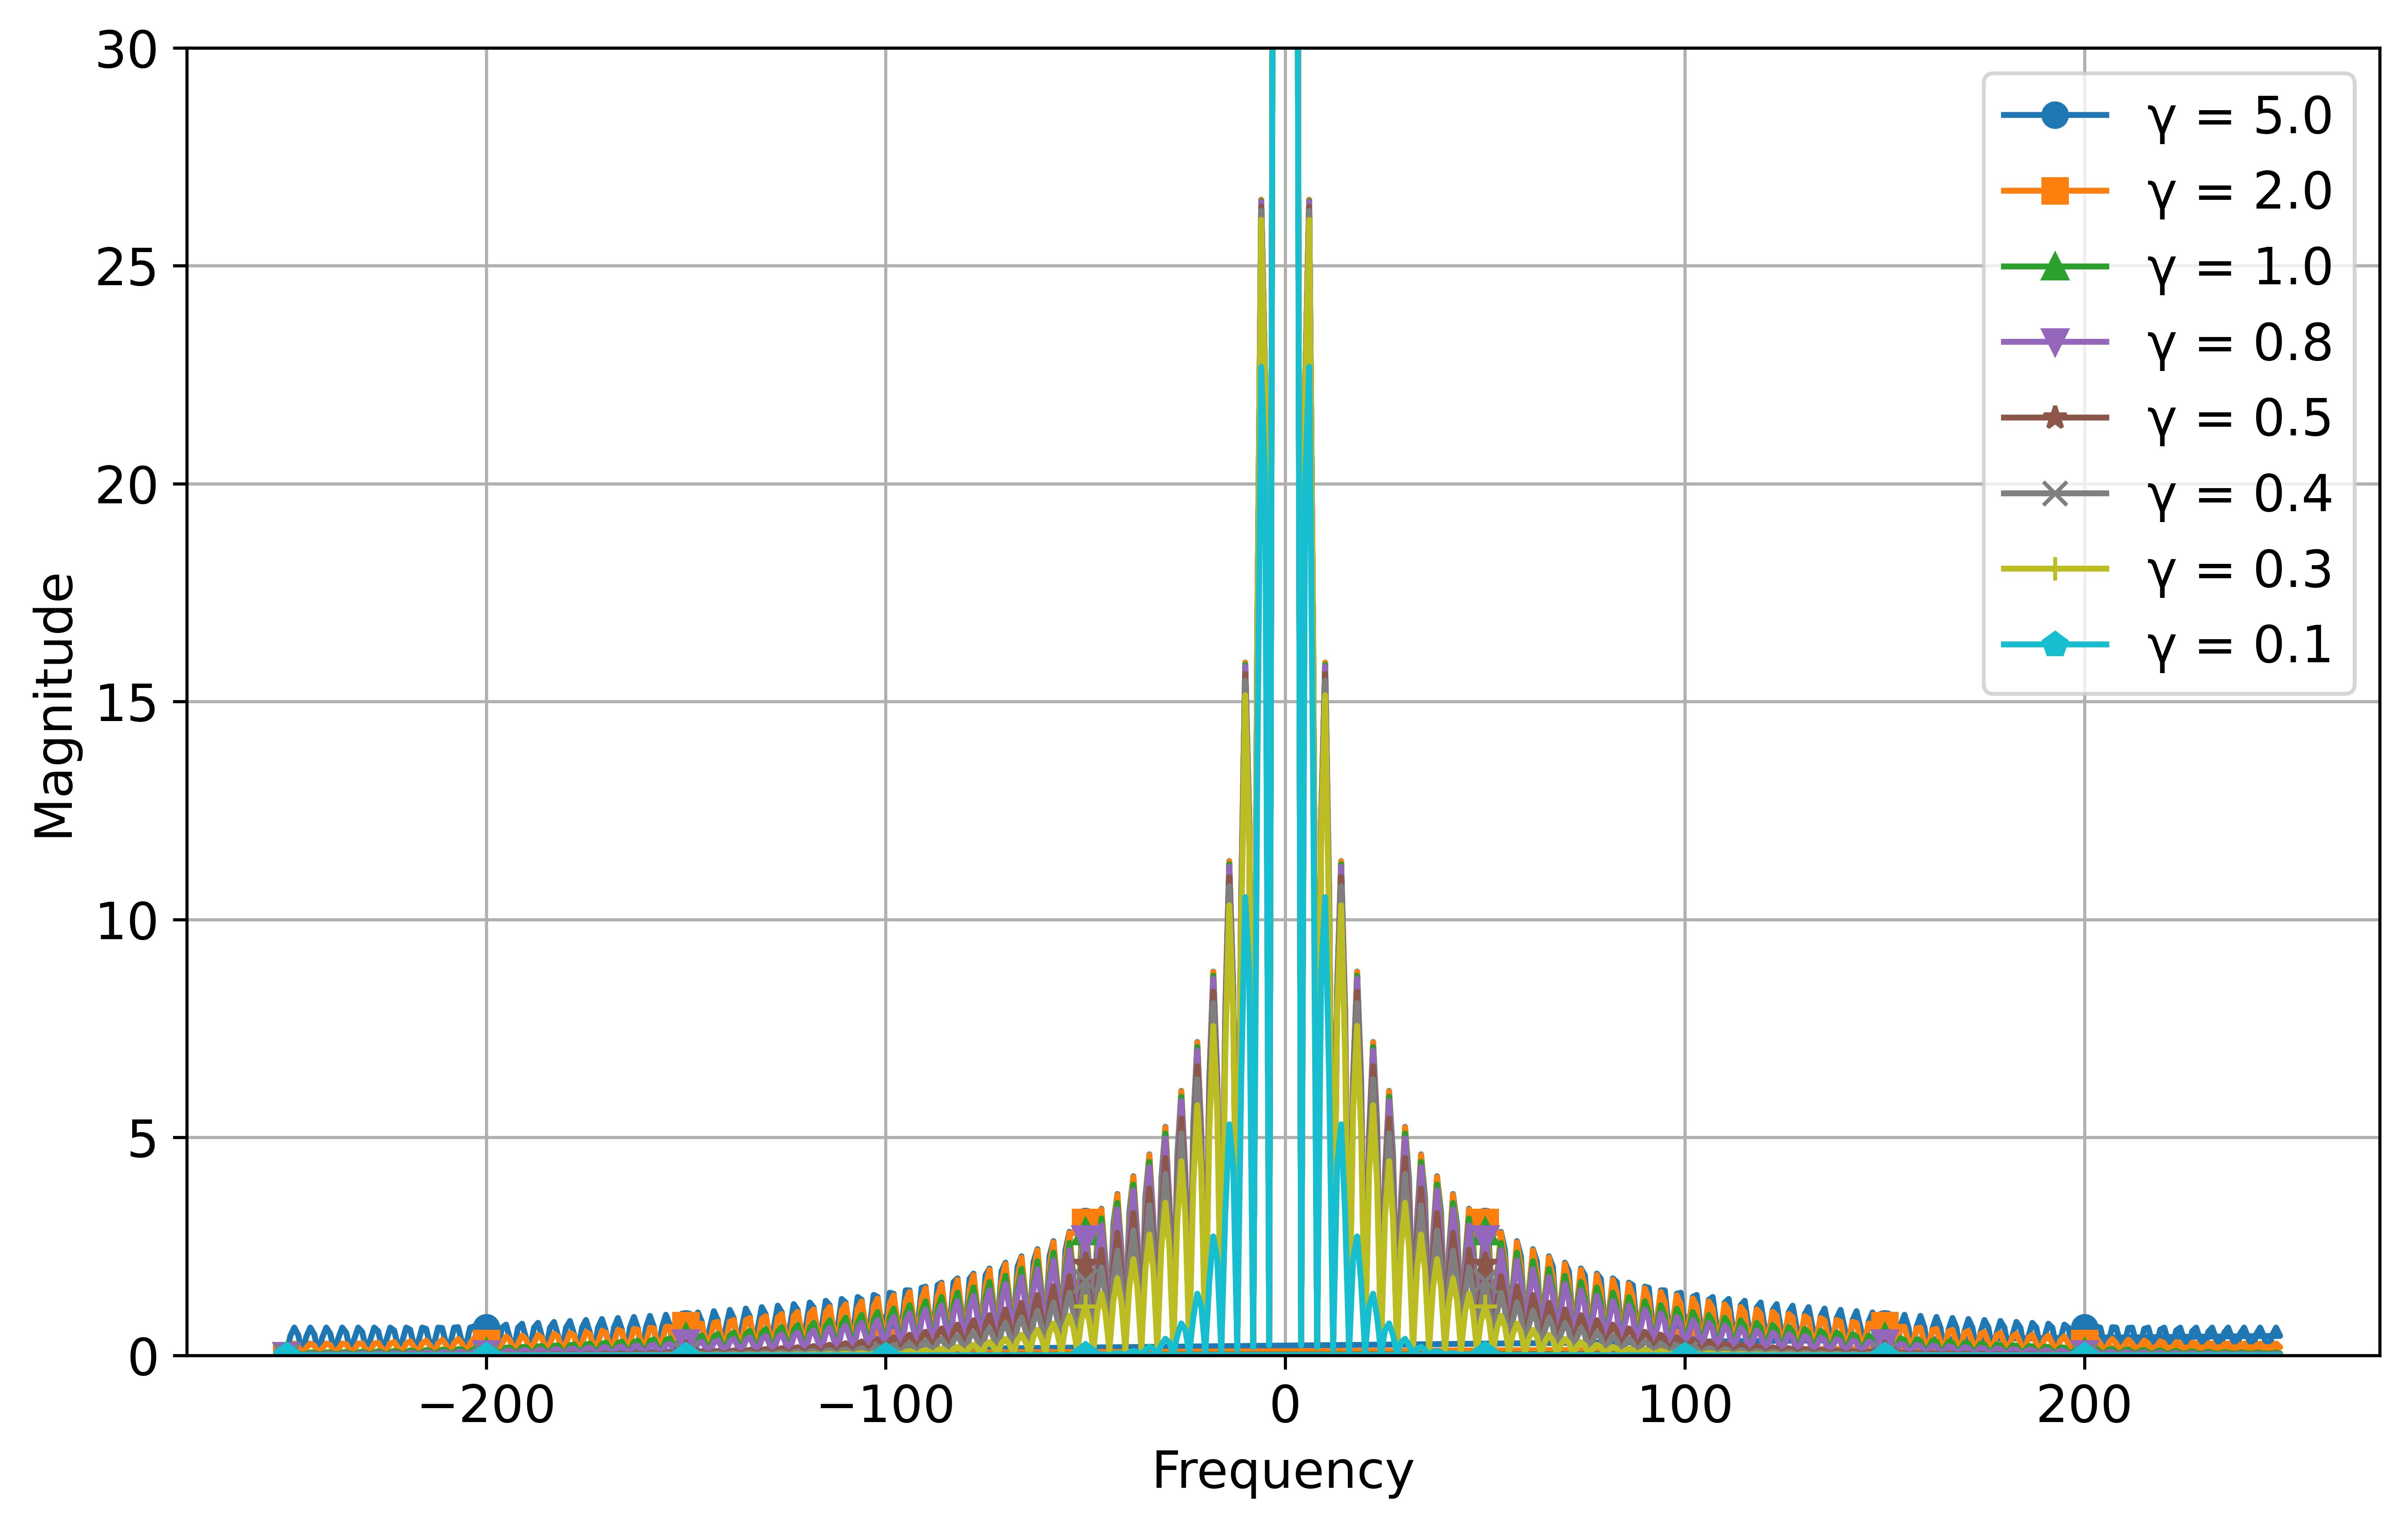
\includegraphics[width=\linewidth]{images/fourieroftophatvarygammaL300.jpg}
  \caption{Fourier Transform of Top-hat Function with Varying $\gamma$, $L_z = 300$}
  \label{fig:fourieroftophatvarygammaL300}
\end{figure}
  
  % \vspace{1em} % Optional spacing between figures

\begin{figure}[htbp]
  \centering
  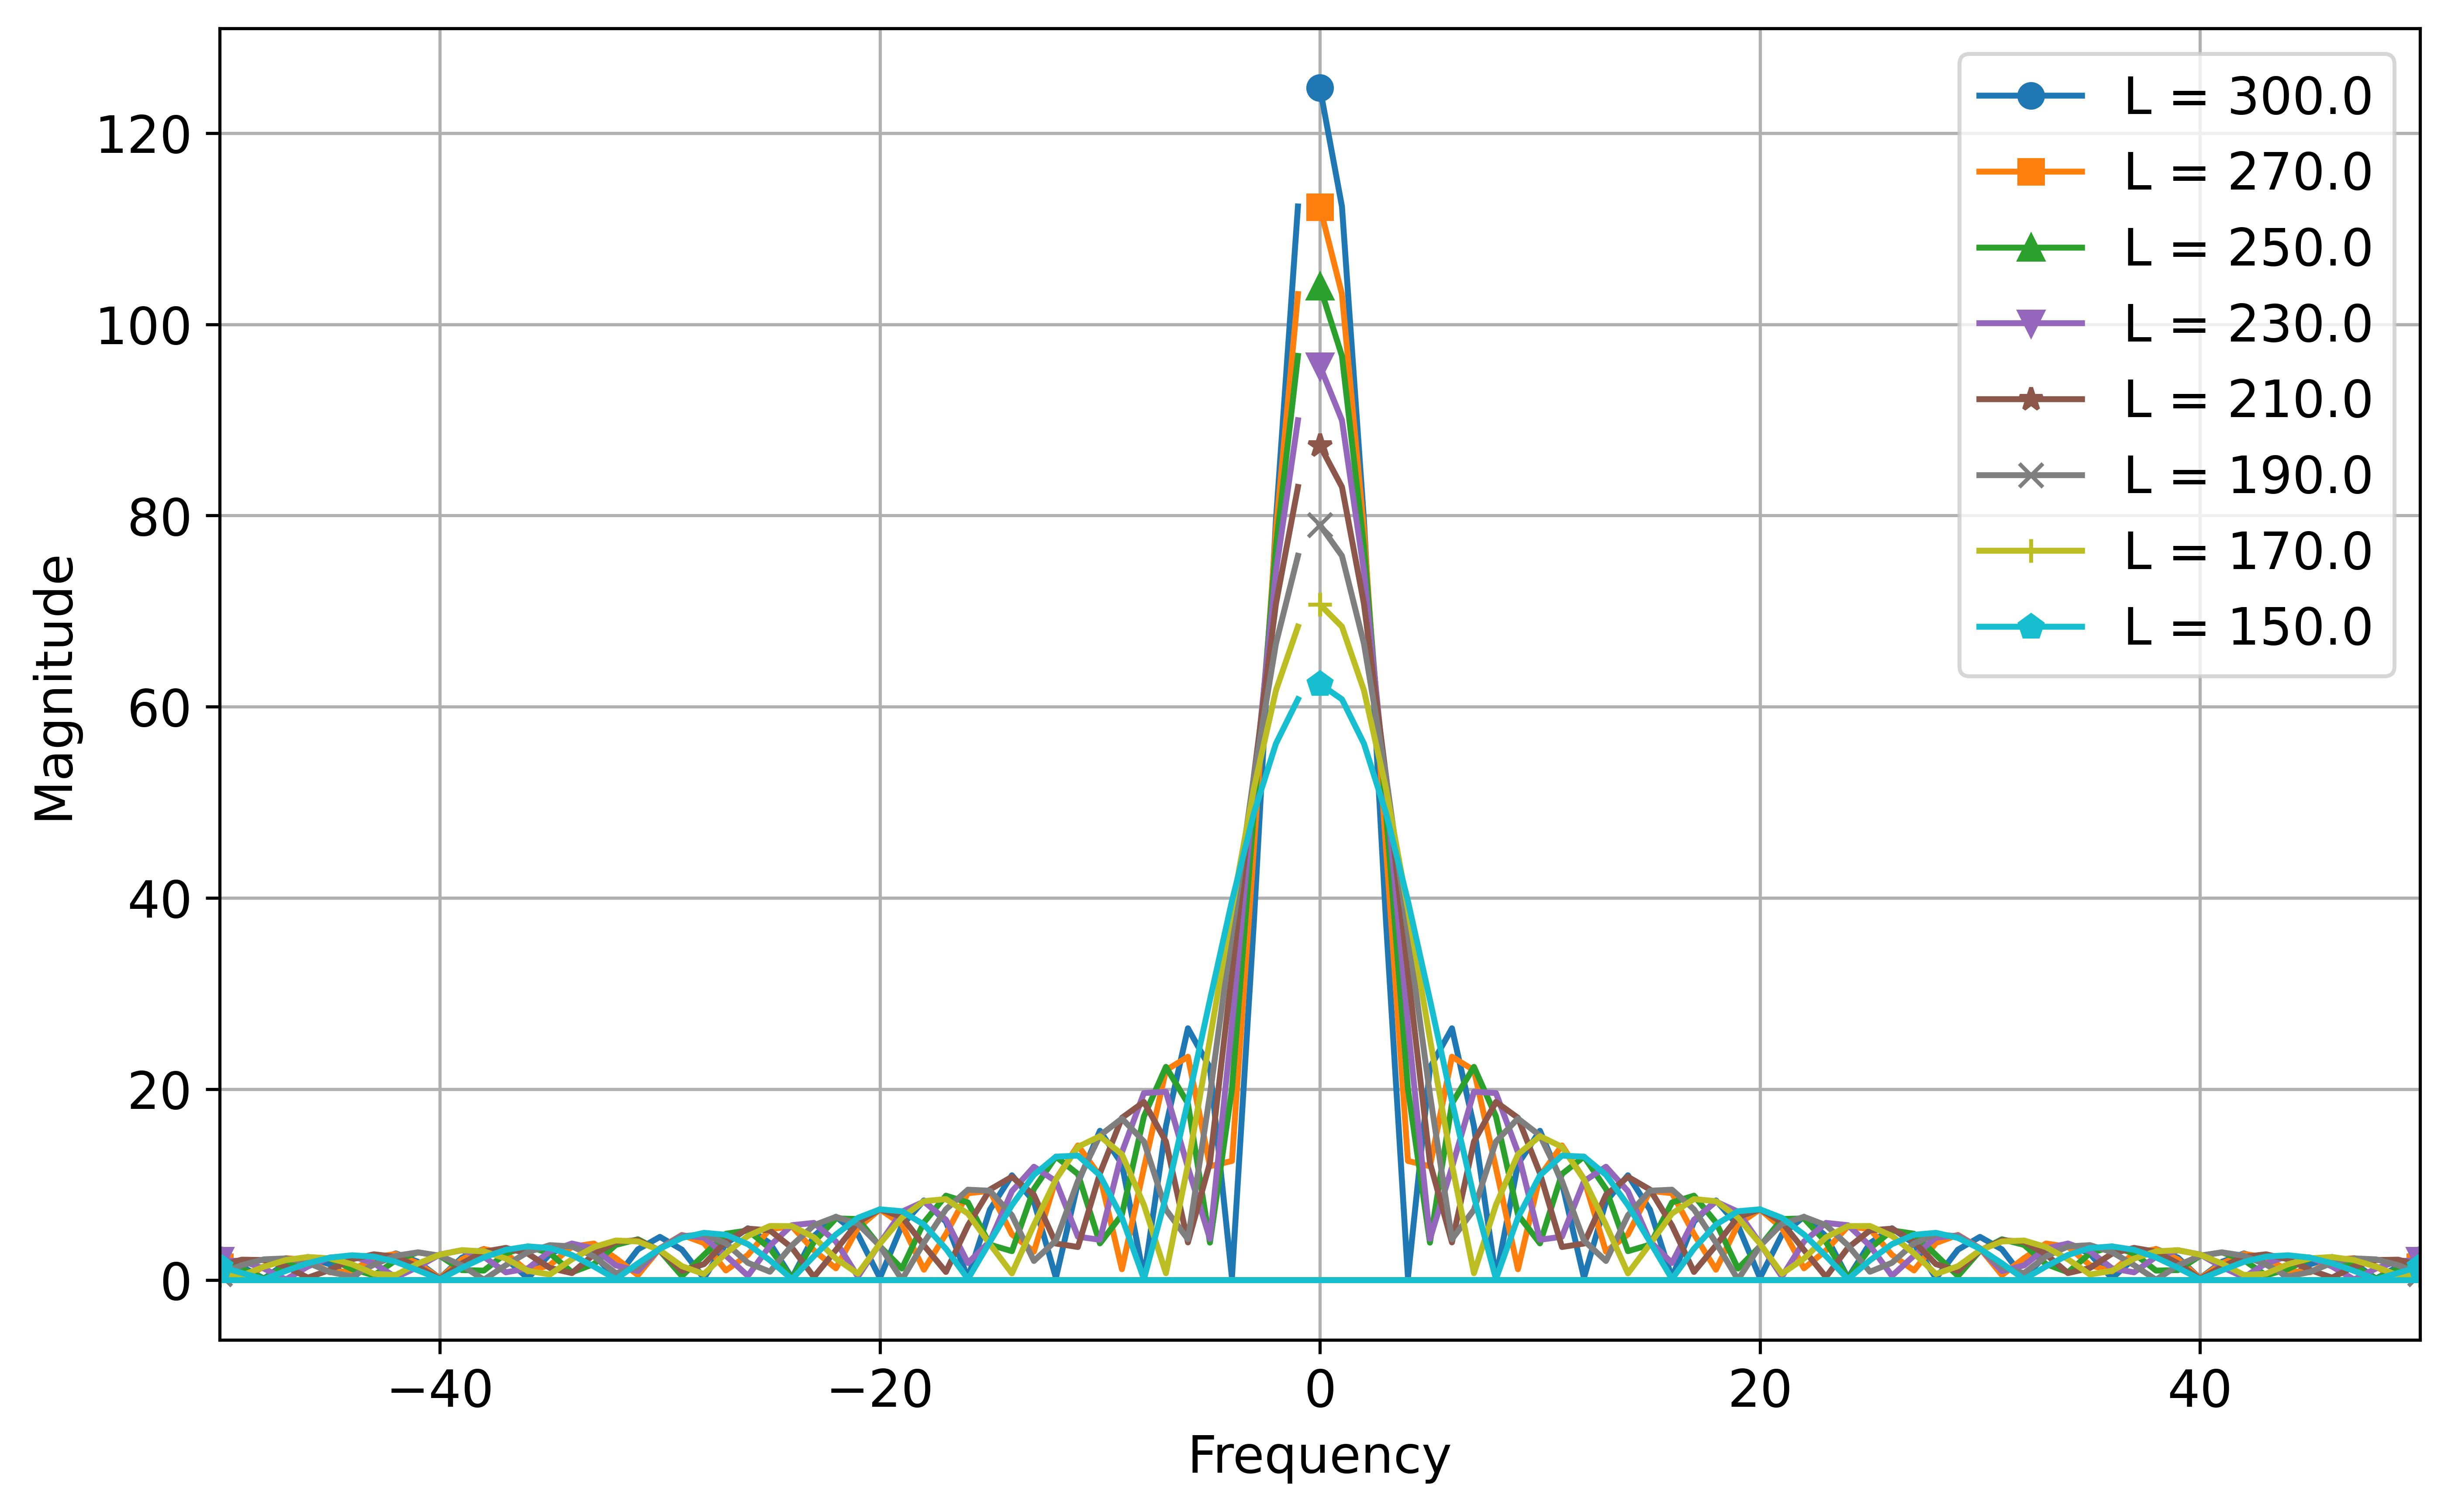
\includegraphics[width=\linewidth]{images/fourieroftophatvaryL_gamma0.5.jpg}
  \caption{Fourier Transform of Top-hat Function with Varying $L_z$, $\gamma = 0.5$}
  \label{fig:fourieroftophatvaryL_gamma0}
\end{figure}

Fig.~(\ref{fig:fourieroftophatvaryL_gamma0}) supports this choice by showing the Fourier Transform for varying $L_z$ at a fixed $\gamma = 0.5$. It demonstrates that changing $L_z$ does not impact the convergence or magnitude of the oscillations in the frequency domain. Although the damping frequency, where oscillations begin to decay, shifts higher with larger $L_z$values, this does not affect the essential behaviour of the transform. This confirms that increasing $L_z$ when using smaller $\gamma$ values does not introduce computational issues, making this a suitable strategy for reducing oscillations while preserving accuracy.

\subsection{Selection of  $L_z$}
To ensure that the simulation cell is completely contained within the region where $\phi(z) = 1$, the smallest possible value for $L_z$ is selected. This approach guarantees the proper placement of the simulation cell and reduces the number of grid points required for the smooth particle mesh Ewald (SPME) method, thereby enhancing computational efficiency. To ascertain the optimal value of $L_z$, a binary search-based algorithm (refer to \textbf{Alg. \ref{alg:vacuum}}) was implemented to determine the box length. Here, the midpoints within a predefined range are checked, and then by repeatedly narrowing the interval, the algorithm quickly converges on the optimal value. This approach reduces the search space \textit{logarithmically}, significantly decreasing the number of evaluations required.

Table~\ref{tab:Lz_values} lists the values of $L_z$ obtained for different decay parameters $\gamma$. As $\gamma$ increases, the decay of the external potential becomes sharper, leading to a more confined region in which $\phi(z) = 1$. 

\begin{algorithm}[htbp]
\caption{Binary Search to Find Simulation Box Vacuum}
\label{alg:vacuum}
\KwData{Side Length: $L > 0$, gamma: $\gamma$}
\KwResult{Optimum vacuum for simulation box}
\textbf{Input:} Side Length: $L$, gamma: $\gamma$, \textbf{Optional: }margin = 5, maxVacuum = 1000 \\
$\text{low} \gets 2 \times L$,
$\text{high} \gets \text{maxVacuum}$

\While{$\text{high} - \text{low} > 1$}{
    $\text{mid} \gets \frac{\text{low} + \text{high}}{2}$ \;
    \If{$\text{tophat}(L, \gamma, \text{mid}) == 1$}{
        $\text{high} \gets \text{mid}$ \;
    }
    \Else{
        $\text{low} \gets \text{mid}$ \;
    }
}
\Return $\text{margin} + \text{high} $\;
\end{algorithm}
\begin{table}[H]
\centering
\caption{Optimized values of box length $L_z$ for various values of the parameter $\gamma$. Smaller values of $\gamma$ correspond to more gradual decay profiles, requiring larger simulation cells while still maintaining $\phi(z) = 1$ within the entire box.}
\label{tab:Lz_values}
\begin{tabular}{|c|c|}
\hline
\rowcolor[HTML]{CBCEFB} 
$\gamma$ & $L_z$ (\AA) \\ \hline
0.2            & 422.5           \\ \hline
0.5            & 202.5           \\ \hline
1              & 129.2           \\ \hline
2.5            & 84.7            \\ \hline
10             & 62.4            \\ \hline
\end{tabular}
\end{table}
